\chapter{Operating System Layer: In-network Near-Memory Processing}
\label{chap:os}
In the previous chapter, we explored the design of memory management for disaggregated architecture at the service layer. However, integrating general applications(other than serverless data analytics) with an external memory service(e.g., Jiffy) requires massive rewrite to integrate with it's API. In this chapter, we instead follow the classic design principles of operating systems and retain memory management functionality within the OS itself. OS manages memory transparently, making it possible to migrate existing data center applications to a disaggregated architecture.

\section{Background: In-network OS design}

Despite the increased interest in memory disaggregation from both academia~\cite{memdisagg2, memdisagg3, memdisagg4, memdisagg5, memdisagg6, memdisagg1, legoos, infiniswap, fastswap, disagg, disaggfault} and industry~\cite{industry0, industry1, industry2, industry3, industry4, industry5}, memory disaggregation still faces three major challenges. First, remote memory access must have low latency and high throughput, with targets of $10~\mu$s latency and $100$ Gbps bandwidth per compute blade~\cite{legoos, infiniswap, fastswap, disagg}. Second, both compute and memory resources need to scale elastically. Finally, adoption requires support for unmodified applications.

We introduce \mind, the first memory management system for rack-scale disaggregated memory that meets all three requirements. \mind places the \mmm within the network fabric, treating the network as a CPU-memory interconnect. By using programmable network switches~\cite{progswitch1, progswitch2, progswitch3} as MMUs, \mind enables a high-performance shared memory abstraction with minimal latency and bandwidth overheads through line-rate processing~\cite{progswitch1}.

To meet the three requirements of memory disaggregation, \mind effectively navigates the constraints of programmable switches and leverages their capabilities for in-network memory management by redesigning traditional memory management as follows:
\begin{itemize}
  \item \textbf{Global Virtual Address Space}: \mind employs a globally shared virtual address space, range-partitioned across memory blades, minimizing the number of address translation entries stored in switch ASIC on-chip memory. Additionally, it uses a load-balancing physical memory allocation mechanism to optimize memory throughput across memory blades.
  
  \item \textbf{Domain-Based Memory Protection}: Inspired by capability-based schemes~\cite{capabilityaddr, cap, opal}, \mind decouples memory permissions from address translation entries, enabling fine-grained, flexible protection while reducing on-chip memory overhead on the switch ASIC.
  
  \item \textbf{Cache Coherence via Directory-Based MSI}: \mind adapts directory-based MSI coherence~\cite{msi} to the in-network environment and uses network-centric hardware primitives like switch ASIC multicast to minimize network overhead in its coherence protocol.
  
  \item \textbf{Dynamic Memory Region Sizing}: To address the challenge of limited switch ASIC memory, \mind tracks memory regions at coarse granularity, which can cause performance degradation from false invalidations. \mind mitigates this with a novel sizing algorithm that dynamically adjusts region sizes, balancing storage efficiency and minimizing performance losses due to false invalidations.
\end{itemize}

\begin{table}
    \caption[Parallels between memory \& networking primitives]{\small \textbf{Parallels between memory \& networking primitives.}}
    \label{table:isomorph}
    \centering
    \scriptsize
    \renewcommand{\arraystretch}{1.2}
    \begin{tabular}{p{3cm} p{1cm}p{3cm}}
      \hline
      \textbf{Virtual Memory} &$\Longleftrightarrow$ &\textbf{Networking} \\\hline\hline
      Memory allocation&&IP assignment\\
      Address translation &&IP forwarding\\
      Memory protection  &&Access control\\
      Cache invalidations &&Multicast\\
      \hline
    \end{tabular}
\end{table}

\subsection{\mind Overview}
\label{ssec:mindoverview}

\begin{figure*}[!t]
\centering
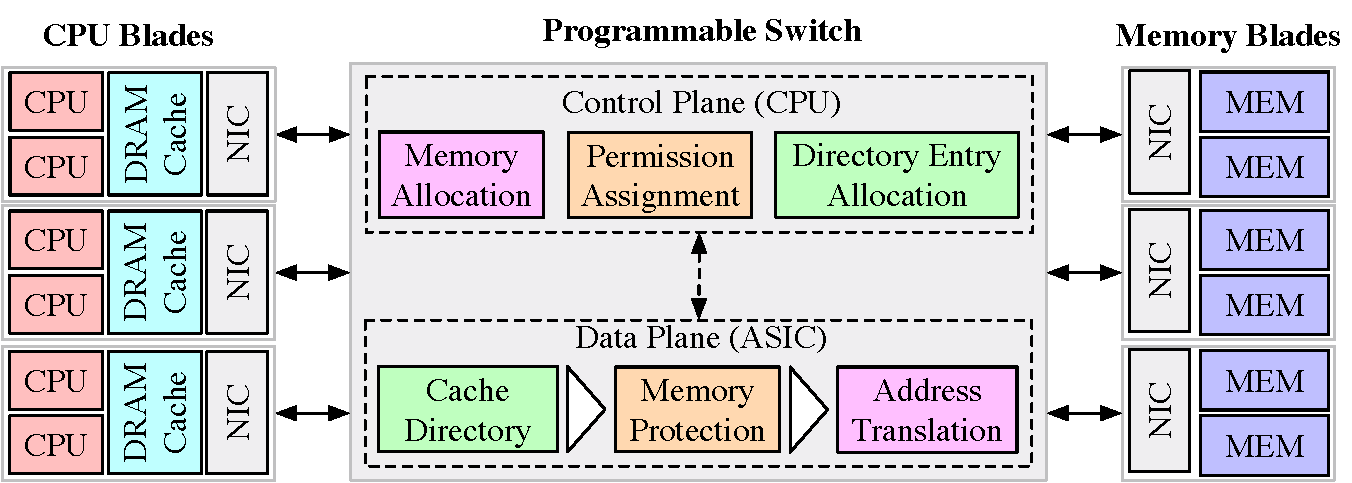
\includegraphics[width=0.55\textwidth]{fig/mind/design}\hspace{3em}
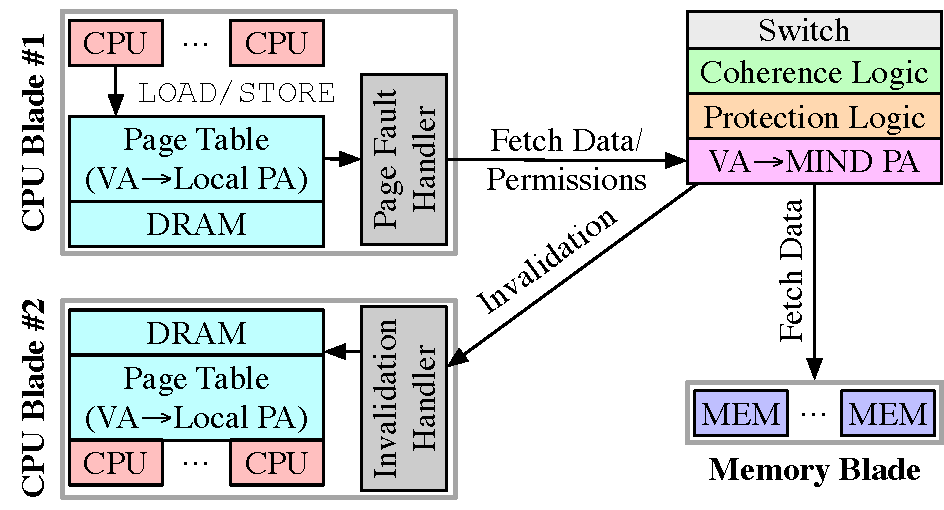
\includegraphics[width=0.35\textwidth]{fig/mind/data_flow}%\vspace{-1em}
\vspace{-0.5em}
\caption[High-level \mind architecture and data flow for memory accesses in \mind]{\textbf{(left) High-level \mind architecture, and, (right) data flow for memory accesses in \mind.}}
\label{fig:system_diagram}
\end{figure*}

We place memory management \textit{in the network fabric} for three reasons.
First, the network fabric enjoys a central location in the disaggregated architecture. Therefore, placing memory management in the data access path between compute and memory resources obviates the need for metadata coherence. 
Second, modern network switches~\cite{progswitch1, progswitch2, progswitch3} permit the implementation of such logic in integrated programmable ASICs. We show that these ASICs are capable of executing it at line rate even for multi-terabit traffic. In fact, many memory management functionalities have similar counterparts in networking (\autoref{table:isomorph}), allowing us to leverage decades of innovation in network hardware and protocol design for disaggregated memory management.
Finally, placing the cache coherence logic and directory in the network switch permits the design of specialized in-network coherence protocols with reduced network latency and bandwidth overheads. 

Effective in-network memory management requires: (\text{i}) \emph{efficient storage}, by  minimizing in-network metadata given the limited memory on the switch data plane;  (\textit{ii}) \emph{high memory throughput}, by load-balancing memory traffic across memory blades; (\textit{iii}) \emph{low access latency to shared memory}, via efficient cache coherence design that hides the network latency.


\subsubsection{Design Overview}
\label{sssec:design}

\mind exposes a \textit{transparent virtual memory} abstraction to applications, similar to server-based OSes. Unlike prior disaggregated memory designs, \mind places all \mmm in the network, instead of CPU or memory blades~\cite{infiniswap, fastswap}, or a separate global controller~\cite{legoos}. 

Figure~\ref{fig:system_diagram}~(left) provides an overview of \mind design, while Figure~\ref{fig:system_diagram}~(right) depicts the data flow for memory accesses in \mind. The \textit{CPU blades} run user processes and threads, and possess a small amount of local DRAM that is used as a cache. All memory allocations (\eg, via \texttt{mmap} or \texttt{sbrk}) and deallocations (\eg, via \texttt{munmap}) from the user processes are intercepted at the CPU blade, and forwarded to the \textit{switch control plane}. The control plane possesses a global view of the system, which it leverages to perform memory allocations, permission assignments and respond to the user process. All memory \code{LOAD}/\code{STORE} operations from the user processes are handled by the CPU blade cache. The cache is virtually addressed\footnote{Note that while it is hidden from applications, CPU blades maintain a local page-based virtual memory abstraction to translate \mind virtual addresses to physical addresses for cached pages in local DRAM (Figure~\ref{fig:system_diagram}~(right)).}, and stores permissions for cached pages to enforce memory protection. If a page is not locally cached, the CPU blade triggers a page-fault and fetches the page from \textit{memory blades} using RDMA requests, evicting other cached pages if necessary. Similarly, if the memory access requires an update to a cached block's coherence state (\eg, \code{STORE} on a Shared or \textbf{S} block), a page-fault is triggered to initiate cache coherence logic at the switch. Note that the page-fault based design requires \mind to perform page-level remote accesses, although future CPU architectures may enable more flexible access granularities.

Since the CPU blade does not store memory management metadata, the RDMA requests are for virtual addresses and do not contain endpoint information (\eg, IP address) for the memory blade that holds the page. Consequently, the \textit{switch data plane} intercepts these requests. It then performs necessary cache coherence logic, including lookups/updates to the cache directory and cache invalidations on other CPU blades. In parallel, the data plane also ensures the requesting process has permissions to access the requested page. If no CPU blade cache holds the page, the data plane translates the virtual addresses to physical addresses, forwarding the request to the appropriate memory blade. 

In \mind's design, the memory blades simply store the actual memory pages, and serve RDMA requests for physical pages. Unlike prior works that employ RPC handlers and polling threads~\cite{legoos}, \mind leverages one-sided RDMA operations~\cite{farm} to obviate the need for any CPU cycles on the disaggregated memory blades. This is a step towards true hardware resource disaggregation, where memory blades need no longer be equipped with any general-purpose CPUs.

\subsection{\mind Design}
\label{ssec:minddesign}

Placing memory management logic and metadata in the network provides the opportunity for simultaneously achieving memory performance and resource elasticity. We now describe how \mind optimizes for the individual goals of memory allocation and addressing (\S\ref{subsec:addr_trans}), memory protection (\S\ref{subsec:mem_prot}), and cache coherence (\S\ref{ssec:caching}), while operating under the constraints of programmable switches. Finally, we detail how \mind handles failures (\S\ref{subsec:acking}). 

\subsubsection{Memory Allocation \& Addressing}
\label{sssec:addr_trans}

Traditional virtual memory uses fixed sized pages as the basic units for both translation and protection; as a result, it cannot achieve the goal of storage efficiency without increasing memory fragmentation: small pages reduce memory fragmentation but require more translation entries, and vice versa.  Following \textbf{P1}, \mind overcomes this by \textit{decoupling} address translation and protection.  That is, \mind's translation is blade-based while protection is \code{vma} based (\S\ref{subsec:mem_prot}).

\paragraphb{Storage-efficient address translation} \mind eschews page-based protection but uses a \textit{single global virtual address-space} across all processes, allowing translation entries to be shared across them. Our approach builds on decades of research on virtual memory designs that also exploit a single address space~\cite{cheri, cap, gam, grappa, opal}, but adds techniques to minimize storage overheads for in-network address translation.
In particular, \mind \textit{range partitions} the virtual address space across different memory blades, such that the entire virtual-address space maps to a contiguous range of physical address space. This allows us to use a single translation entry for each memory blade: any virtual address that falls within its range can be directly routed to that memory blade, minimizing the storage required on switch data plane. In \mind, this mapping only changes when new memory blades join, old ones retire or if memory is moved between blades.

\paragraphb{Balanced memory allocation \& reduced fragmentation} \mind's control plane, leveraging its global view of allocations (\textbf{P2}), tracks the total amount of memory allocated on each memory blade and places a new allocation on the blade with the least allocation, to achieve near-optimal load-balancing. We validate this empirically in \S\ref{sec:evaluation}.

Moreover, since there is a one-to-one mapping between virtual and physical addresses within a particular memory blade, \mind minimizes external fragmentation at each memory blade by using traditional virtual memory allocation schemes that have evolved to facilitate the same, \eg, first-fit allocator in our implementation~\cite{firstfit}.
The result of memory allocation is a virtual memory area (\texttt{vma}), identified by the base virtual address and length of the area, \eg, 
  {{\small <\texttt{0x00007f84b862d33b}, \texttt{0x400}>}}
for a $1$KB area. 
As will be elaborated in \S\ref{subsec:mem_prot}, \code{vma} is the basic unit of protection in \mind.
This allows multiple processes to have non-overlapping \code{vma}s on the same blade, minimizing memory fragmentation.
 
\paragraphb{Isolation} We note that \mindx's global virtual address-space does not compromise on \textit{isolation} between processes. First, since the switch intercepts allocation requests across all compute blades, and possesses a global view of valid allocations at any time, it can easily ensure allocations are non-overlapping across different processes. Second, we show in \S\ref{subsec:mem_prot} that \mind's \code{vma}-based protection allows flexible access control between processes in a single global virtual address-space.

\paragraphb{Transparency via outlier entries} \mindx's one-to-one mapping between virtual and physical addresses does not preclude supporting unmodified applications with static virtual addresses embedded within their binaries, or OS optimizations such as page migration~\cite{pagemigrations}, \ie, moving pages from one memory blade to another. \mind maintains separate \textit{range-based} address translations~\cite{rangetranslations} for physical memory regions that correspond to static virtual addresses or migrated memory. These \textit{outlier} entries are stored succinctly in the switch TCAM, where the TCAM's longest-prefix matching (LPM) property ensures that only the most specific entry (\ie, one with the longest prefix) is considered when translating a virtual address, ensuring correctness.

\subsubsection{Memory Protection}
\label{sssec:mem_prot}

As \mind decouples translation and protection, it uses a separate table to store memory protection entries in the data plane. 
Consequently, an application can assign access permissions to a \code{vma} of any size.
The size of this protection table is proportional to the number of \code{vma}s. We find this number is reasonably small in our experiments and the protection table can easily fit in the switch ASIC even for a wide range of memory-intensive applications (\S\ref{sec:evaluation}). This is because the first-fit allocator and Linux's \code{glibc} allocation requests~\cite{glibc-alloc} do a good job of ensuring \code{vma}s are large and contiguous. 

\paragraphb{Fine-grained, flexible memory protection} Similar to prior work on capability-based systems~\cite{cheri, capabilityaddr}, \mind supports two key abstractions: \textit{protection domains} and \textit{permission classes}. Protection domains identify the entity that may (or may not) have permissions to access a particular memory region of arbitrary size, while the permission class identifies what the entity can do to the memory region. 
\mind's control plane exposes a set of APIs for memory allocation and permission changes that allows an application to specify a protection domain identifier (\code{PDID}) for an arbitrary virtual memory area (\code{vma}) and assign a permission class (\code{PC}) to the pair \code{<PDID}, \code{vma>}. 
The mapping \code{<PDID}, \code{vma>} $\rightarrow$ \code{PC} is stored as an entry in the protection table in the data plane. For existing applications, \mind simply takes the process identifier (\code{PID}) as the \code{PDID},  and uses Linux memory permissions (\eg, read-only, read-write, \etc) as permission classes. Note that \mind \textit{can} support richer memory protection semantics than traditional OSes, \eg, user programs that serve multiple client sessions, such as ssh servers or database services, can assign a separate protection domain per session to prevent one session from accessing data from other sessions~\cite{cheri}. 

Following principle \textbf{P3}, we leverage TCAM-based parallel range matches in the programmable switch ASIC --- typically used for IP subnet matches --- to efficiently support fine-grained matching for \code{<PDID}, \code{vma>} entries embedded in memory access requests and obtain corresponding the permission class (\code{PC}). If there is a mismatch between \code{PC} and the memory access type, or the \code{<PDID}, \code{vma>} entry does not exist, the request is rejected.

\paragraphb{Optimizing for TCAM storage} One limitation of TCAM is that each of its entries can only match power-of-two ranges. \mind overcomes this by splitting an arbitrary-sized virtual address range into multiple power-of-two-sized entries. Note that the number of entries required for a range of size $s$ is upper-bounded by $\lceil\log_2(s)\rceil$. In order to meet our goal of storage efficiency in the switch data plane, the control plane (1) only performs virtual address allocations that are aligned with the power-of-two sizes to ensure each region can be represented using a single TCAM entry, and (2) coalesces adjacent entries with if they belong to the same protection domain and have the same permission class. Interestingly, memory allocations requested by underlying libraries (\eg, \texttt{glibc}) are mostly in power-of-two sizes anyway, enabling storage-efficiency for TCAM entries.


